Die mobile App wurde mit Flutter entwickelt, um eine plattformübergreifende Verfügbarkeit sowohl für Android als auch für iOS sicherzustellen. Flutter ermöglichte es, eine einzige Codebasis für beide Plattformen zu nutzen, wodurch der Entwicklungsaufwand reduziert und eine konsistente Benutzererfahrung gewährleistet wurde. Diese Entscheidung wurde getroffen, um die App möglichst effizient zu gestalten und gleichzeitig ein breites Publikum zu erreichen.

\subsection{Funktionen der App}
Die App bietet eine Vielzahl von Funktionen, die speziell auf die Verwaltung und Nutzung des Smartenders abgestimmt sind. Sie wurde so konzipiert, dass Benutzer sowohl die Steuerung des Smartenders als auch die Verwaltung von Rezepten und Zutaten übernehmen können. Zu den wichtigsten Funktionen gehören:

\begin{itemize}
    \item \textbf{Rezepte erstellen, ändern und löschen:} Benutzer können eigene Cocktailrezepte anlegen und diese flexibel verwalten.
    \item \textbf{Zutaten hinzufügen, ändern und löschen:} Die App erlaubt die Organisation und Anpassung der verfügbaren Zutaten.
    \item \textbf{Eingesteckte Flaschen (Zutaten) festlegen und ändern:} Es kann definiert werden, welche Zutaten in welchen Slots des Smartenders verfügbar sind.
    \item \textbf{Bestellungen auslösen:} Die App ermöglicht das direkte Auslösen von Cocktailbestellungen am Smartender.
    \item \textbf{Rezepte favorisieren:} Häufig genutzte Rezepte können als Favoriten markiert und schnell abgerufen werden.
    \item \textbf{Light- und Darkmode:} Benutzer können zwischen einem hellen und dunklen Designmodus wechseln, um die App an ihre Präferenzen anzupassen.
\end{itemize}
Die Integration mit einem zentralen Backend sorgt dafür, dass alle Daten synchronisiert und jederzeit auf dem neuesten Stand sind. Dadurch können Benutzer ihre Rezept- und Zutatenlisten von mehreren Geräten aus abrufen und bearbeiten.

\subsection{Benutzeroberfläche (UI) und Design}
Die App verfolgt ein minimalistisches und intuitives Design, das Elemente des Material Designs integriert, ohne ein dediziertes Design-Framework zu nutzen. Das Ziel war es, die Benutzeroberfläche so einfach und zugänglich wie möglich zu gestalten, damit sie auch von technisch weniger erfahrenen Nutzern problemlos bedient werden kann.

Die Struktur der App umfasst mehrere zentrale Bereiche:

\begin{itemize}
    \item \textbf{Login- und Registrierungs-Screens:} Diese erscheinen nur, wenn ein Benutzer sich neu registrieren oder nach einem ausgelaufenen Token erneut einloggen möchte. Dadurch wird der Workflow für eingeloggte Benutzer vereinfacht.
    \item \textbf{Hauptscreens:} Drei Hauptscreens sind über eine Bottom-Navigationsleiste zugänglich:
    \begin{itemize}
        \item \textbf{Rezepte-Screen:} Zeigt eine Liste aller gespeicherten Rezepte an und bietet Optionen zur Bearbeitung oder Löschung.
        \item \textbf{Favoriten-Screen:} Zeigt nur die als Favoriten markierten Rezepte an und ist ähnlich dem Rezepte-Screen aufgebaut.
        \item \textbf{Einstellungen-Screen:} Ermöglicht die Verwaltung von Zutaten und Slots, das Wechseln des Designs zwischen Light- und Darkmode sowie das Ausloggen.
    \end{itemize}
\end{itemize}



\begin{figure}[H]
    \centering
    \begin{minipage}{0.27\textwidth}
        \centering
        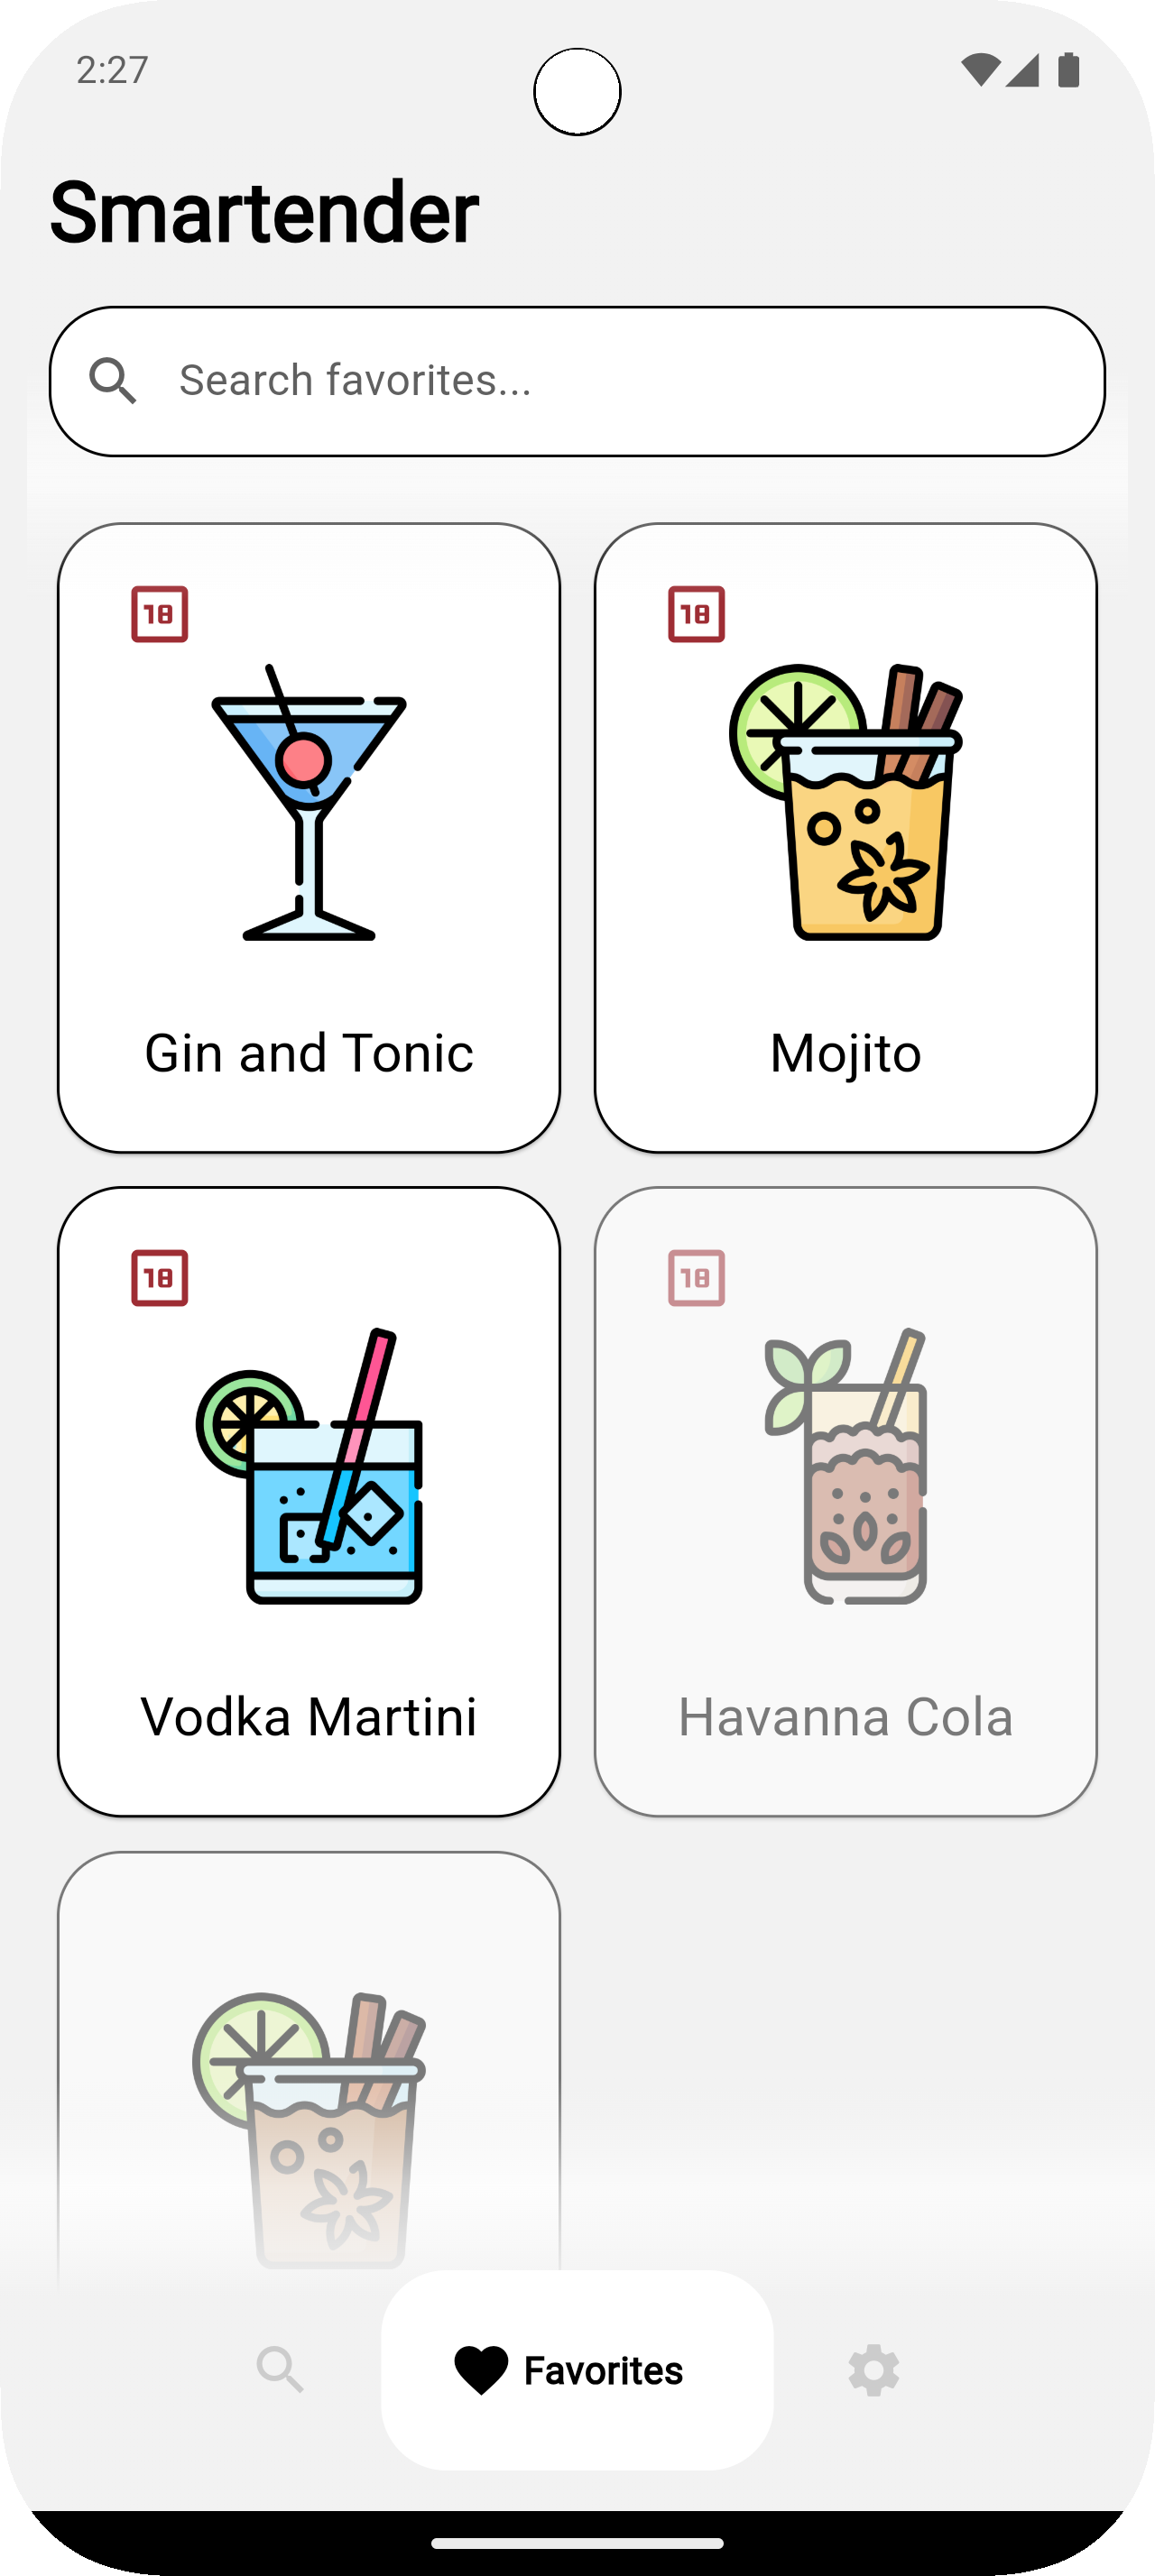
\includegraphics[width=\textwidth]{graphics/images/favorites_light.png}
        \caption{Favoritenansicht im Lightmode}
        \label{fig:favorites_light}
    \end{minipage}
    \hfill
    \begin{minipage}{0.27\textwidth}
        \centering
        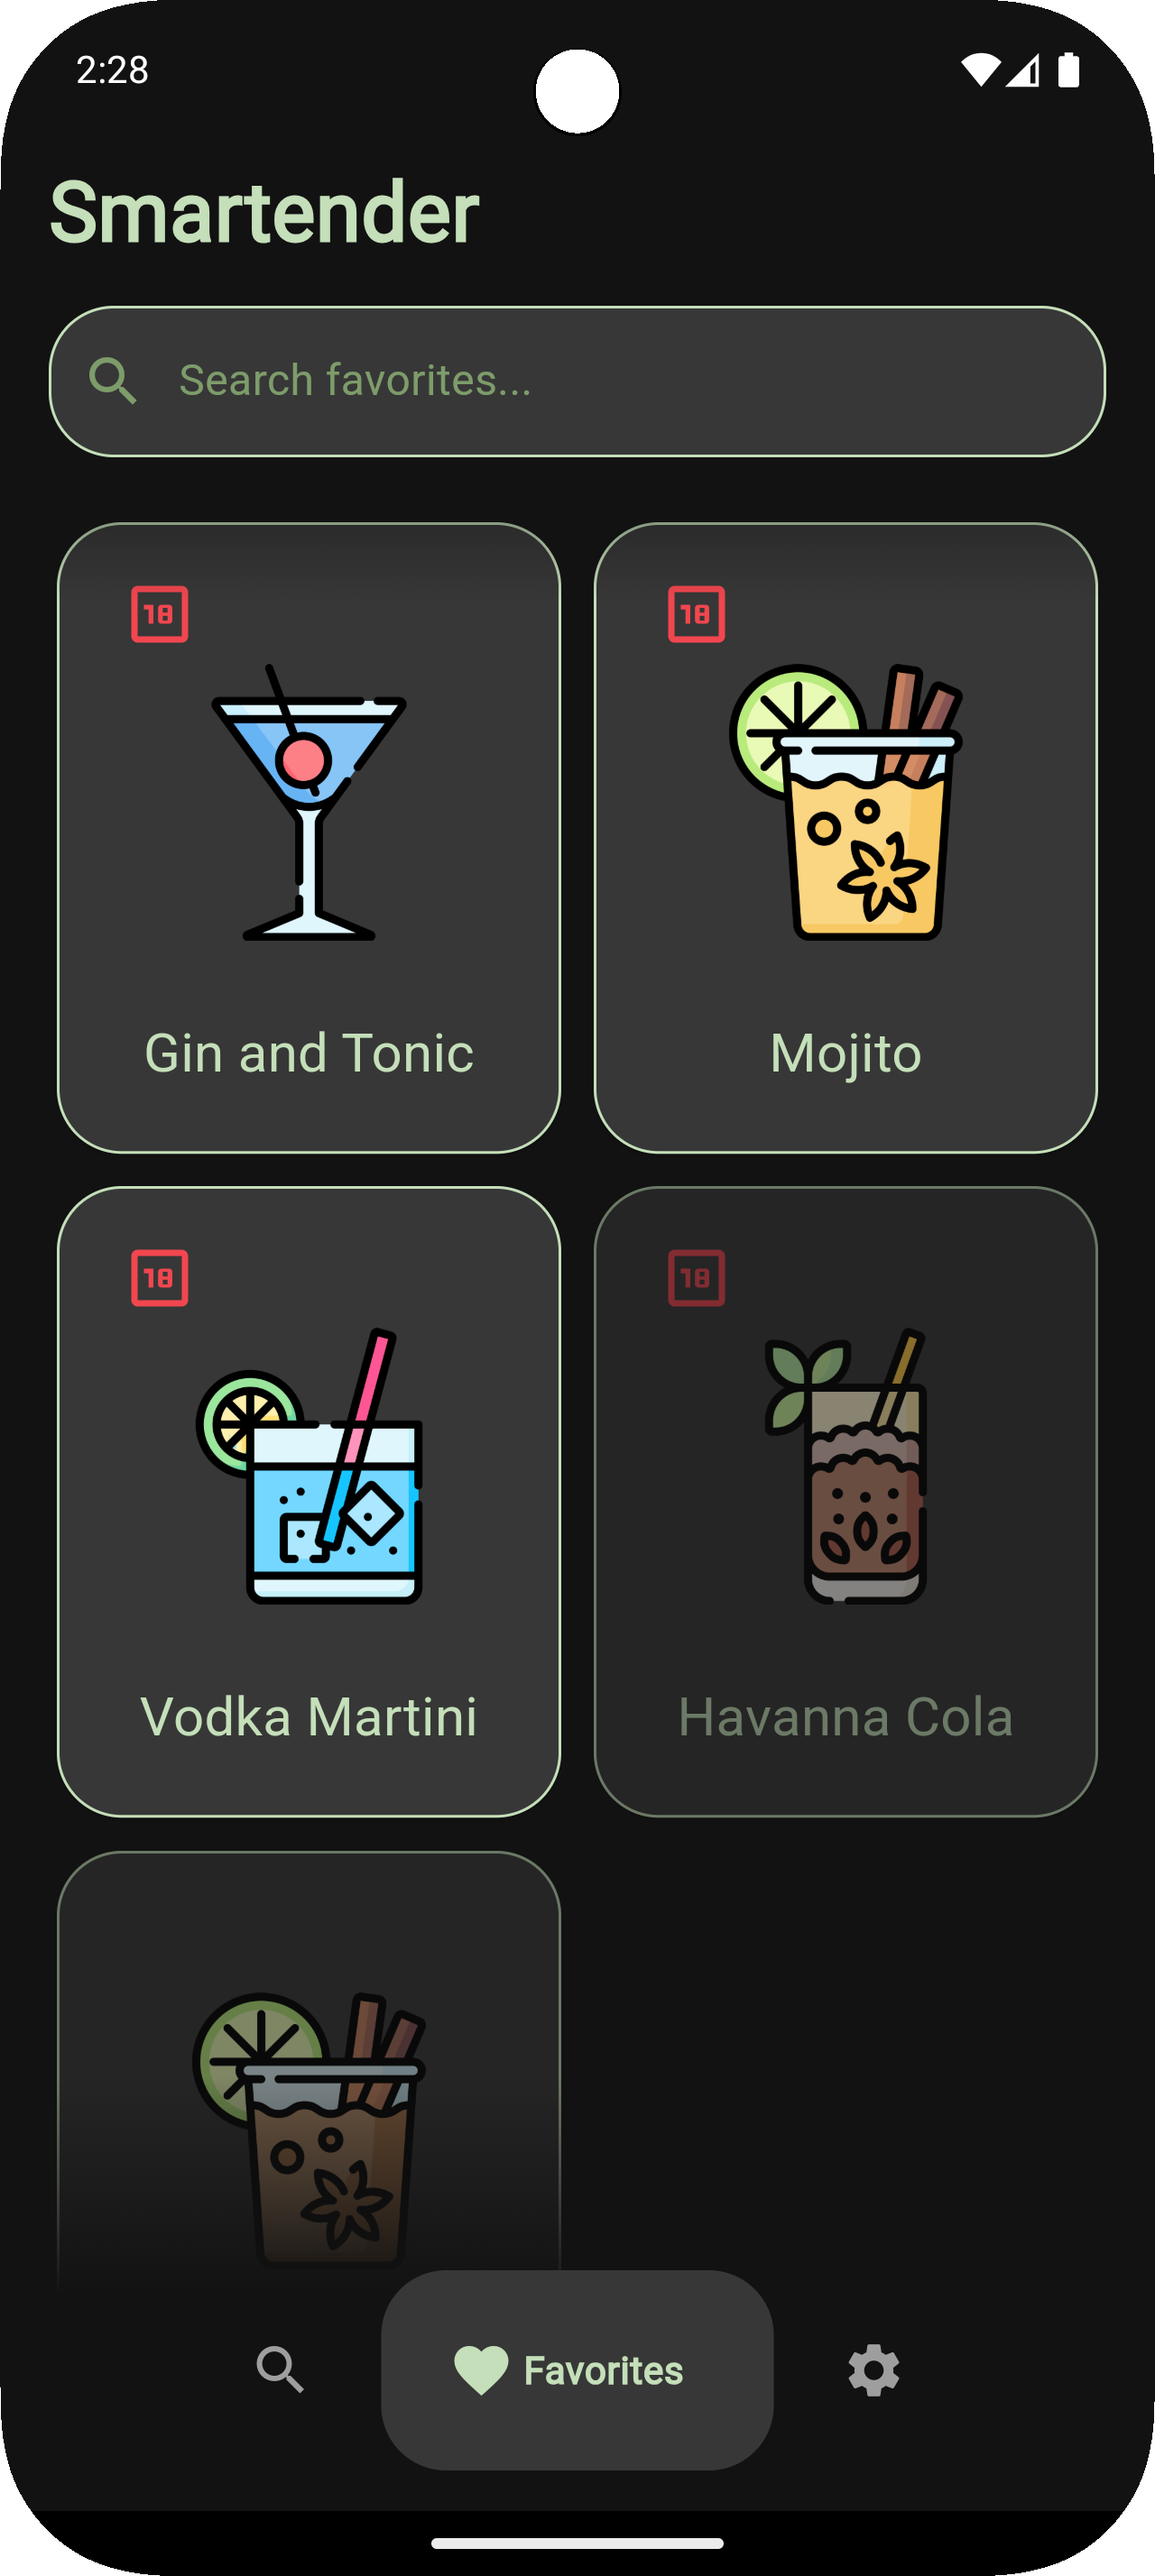
\includegraphics[width=\textwidth]{graphics/images/favorites_dark.png}
        \caption{Favoritenansicht im Darkmode}
        \label{fig:favorites_dark}
    \end{minipage}
    \hfill
    \begin{minipage}{0.27\textwidth}
        \centering
        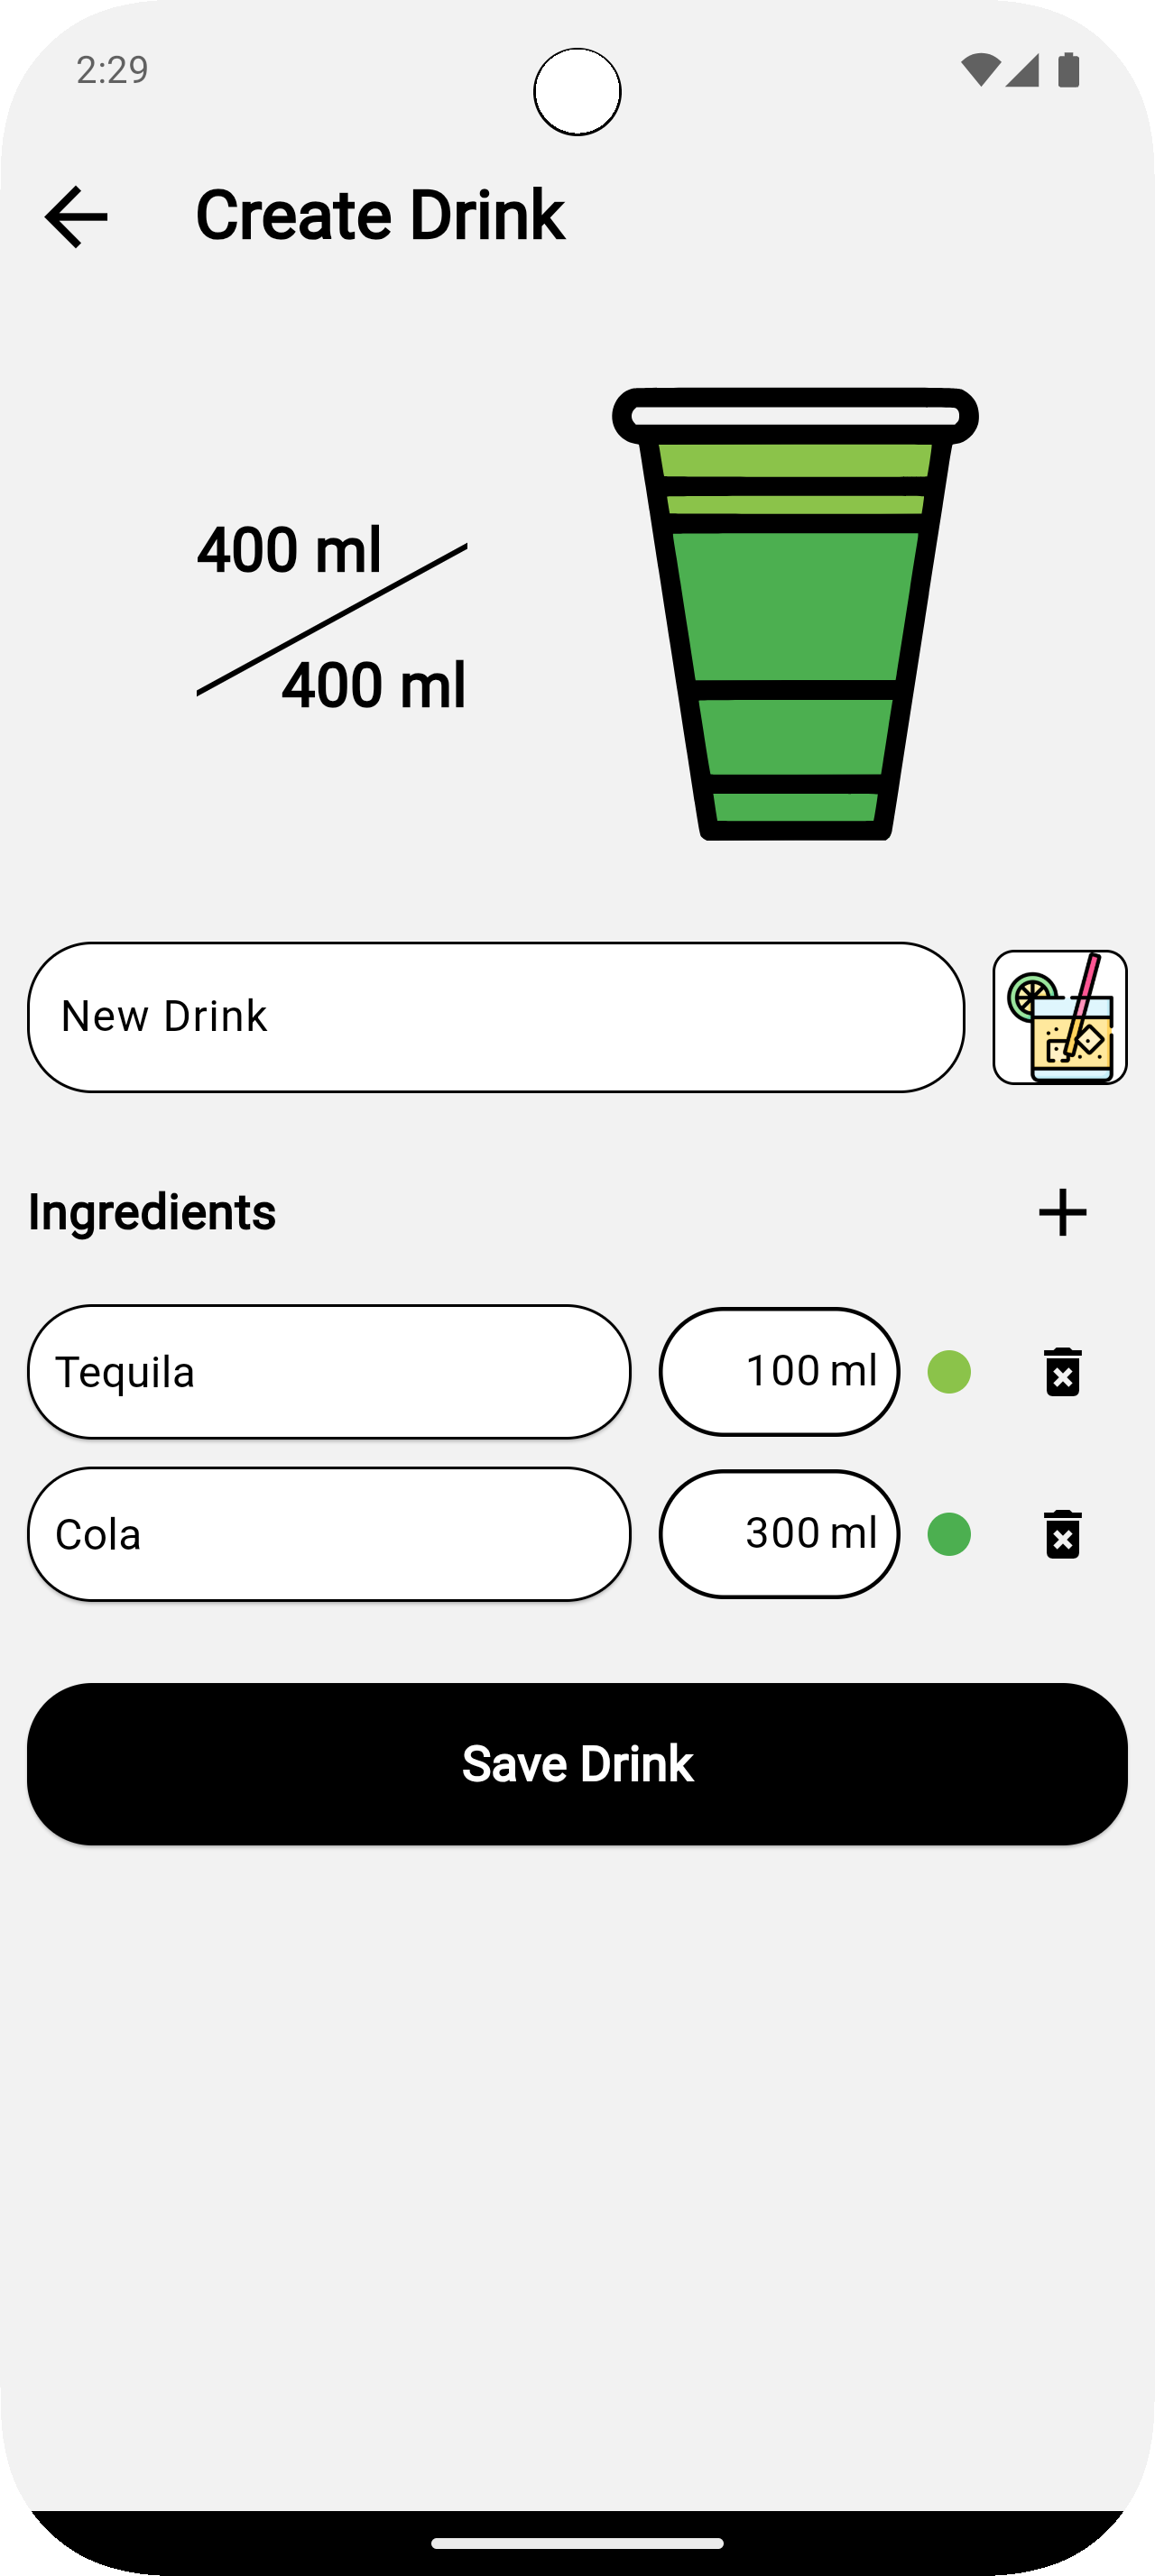
\includegraphics[width=\textwidth]{graphics/images/create_drink.png}
        \caption{Createdrinkscreen im Lightmode}
        \label{fig:create_drink}
    \end{minipage}
    \label{fig:favorites}
\end{figure}



\subsection{Integration und Kommunikation}
Die App kommuniziert über eine REST-API mit dem Backend, wodurch Daten wie Benutzerrezepte, Zutaten und Bestellungen synchronisiert werden. Diese Architektur ermöglicht eine nahtlose Integration und stellt sicher, dass alle Geräte jederzeit auf aktuelle Daten zugreifen können. Die REST-API stellt Endpunkte für folgende Aufgaben bereit:

\begin{itemize}
    \item Abruf und Aktualisierung von Benutzerinformationen
    \item Verwaltung von Rezepten und Zutaten
    \item Auslösen und Überwachung von Bestellungen
\end{itemize}
Eine wichtige Optimierung in der App war die Reduzierung unnötiger Backend-Aufrufe. Ursprünglich wurden Daten alle 10 Sekunden automatisch aktualisiert, was zu einer hohen Serverlast führen konnte. Dies wurde so angepasst, dass die Aktualisierung nur erfolgt, wenn ein Benutzer zwischen den Hauptscreens wechselt. Dadurch konnte die Performance des Systems deutlich verbessert werden.

\subsection{Entwicklungsprozess}
Während der Entwicklung traten einige Herausforderungen auf, insbesondere im Hinblick auf die Anpassung der App an unterschiedliche Bildschirmauflösungen. Obwohl Flutter eine responsive Gestaltung ermöglicht, kam es bei Tests mit einem Samsung S24 Ultra zu einem Overflow-Fehler. Dieser wurde als Einzelfall behandelt, da die App auf anderen Geräten fehlerfrei funktionierte. Zur Entwicklung wurden folgende Tools genutzt:

\begin{itemize}
    \item \textbf{Android Studio:} Hauptentwicklungsumgebung für Android.
    \item \textbf{Postman:} Testen der REST-API-Schnittstellen.
    \item \textbf{Xcode:} Build-Prozess und Tests für iOS-Geräte.
\end{itemize}
Um technische Details zu überprüfen und Designentscheidungen zu bewerten, wurden mehrere Testversionen der App erstellt. Diese wurden unter den Entwicklern getestet, um Fehler zu identifizieren und Verbesserungen vorzunehmen. Dieser iterative Ansatz ermöglichte eine kontinuierliche Optimierung der App.

